\documentclass[]{article}
\usepackage{lmodern}
\usepackage{amssymb,amsmath}
\usepackage{ifxetex,ifluatex}
\usepackage{fixltx2e} % provides \textsubscript
\ifnum 0\ifxetex 1\fi\ifluatex 1\fi=0 % if pdftex
  \usepackage[T1]{fontenc}
  \usepackage[utf8]{inputenc}
\else % if luatex or xelatex
  \ifxetex
    \usepackage{mathspec}
    \usepackage{xltxtra,xunicode}
  \else
    \usepackage{fontspec}
  \fi
  \defaultfontfeatures{Mapping=tex-text,Scale=MatchLowercase}
  \newcommand{\euro}{€}
\fi
% use upquote if available, for straight quotes in verbatim environments
\IfFileExists{upquote.sty}{\usepackage{upquote}}{}
% use microtype if available
\IfFileExists{microtype.sty}{%
\usepackage{microtype}
\UseMicrotypeSet[protrusion]{basicmath} % disable protrusion for tt fonts
}{}
\usepackage[margin=1in]{geometry}
\ifxetex
  \usepackage[setpagesize=false, % page size defined by xetex
              unicode=false, % unicode breaks when used with xetex
              xetex]{hyperref}
\else
  \usepackage[unicode=true]{hyperref}
\fi
\hypersetup{breaklinks=true,
            bookmarks=true,
            pdfauthor={},
            pdftitle={Exploratory Data Analysis Using the ToothGrowth Dataset},
            colorlinks=true,
            citecolor=blue,
            urlcolor=blue,
            linkcolor=magenta,
            pdfborder={0 0 0}}
\urlstyle{same}  % don't use monospace font for urls
\usepackage{color}
\usepackage{fancyvrb}
\newcommand{\VerbBar}{|}
\newcommand{\VERB}{\Verb[commandchars=\\\{\}]}
\DefineVerbatimEnvironment{Highlighting}{Verbatim}{commandchars=\\\{\}}
% Add ',fontsize=\small' for more characters per line
\usepackage{framed}
\definecolor{shadecolor}{RGB}{248,248,248}
\newenvironment{Shaded}{\begin{snugshade}}{\end{snugshade}}
\newcommand{\KeywordTok}[1]{\textcolor[rgb]{0.13,0.29,0.53}{\textbf{{#1}}}}
\newcommand{\DataTypeTok}[1]{\textcolor[rgb]{0.13,0.29,0.53}{{#1}}}
\newcommand{\DecValTok}[1]{\textcolor[rgb]{0.00,0.00,0.81}{{#1}}}
\newcommand{\BaseNTok}[1]{\textcolor[rgb]{0.00,0.00,0.81}{{#1}}}
\newcommand{\FloatTok}[1]{\textcolor[rgb]{0.00,0.00,0.81}{{#1}}}
\newcommand{\ConstantTok}[1]{\textcolor[rgb]{0.00,0.00,0.00}{{#1}}}
\newcommand{\CharTok}[1]{\textcolor[rgb]{0.31,0.60,0.02}{{#1}}}
\newcommand{\SpecialCharTok}[1]{\textcolor[rgb]{0.00,0.00,0.00}{{#1}}}
\newcommand{\StringTok}[1]{\textcolor[rgb]{0.31,0.60,0.02}{{#1}}}
\newcommand{\VerbatimStringTok}[1]{\textcolor[rgb]{0.31,0.60,0.02}{{#1}}}
\newcommand{\SpecialStringTok}[1]{\textcolor[rgb]{0.31,0.60,0.02}{{#1}}}
\newcommand{\ImportTok}[1]{{#1}}
\newcommand{\CommentTok}[1]{\textcolor[rgb]{0.56,0.35,0.01}{\textit{{#1}}}}
\newcommand{\DocumentationTok}[1]{\textcolor[rgb]{0.56,0.35,0.01}{\textbf{\textit{{#1}}}}}
\newcommand{\AnnotationTok}[1]{\textcolor[rgb]{0.56,0.35,0.01}{\textbf{\textit{{#1}}}}}
\newcommand{\CommentVarTok}[1]{\textcolor[rgb]{0.56,0.35,0.01}{\textbf{\textit{{#1}}}}}
\newcommand{\OtherTok}[1]{\textcolor[rgb]{0.56,0.35,0.01}{{#1}}}
\newcommand{\FunctionTok}[1]{\textcolor[rgb]{0.00,0.00,0.00}{{#1}}}
\newcommand{\VariableTok}[1]{\textcolor[rgb]{0.00,0.00,0.00}{{#1}}}
\newcommand{\ControlFlowTok}[1]{\textcolor[rgb]{0.13,0.29,0.53}{\textbf{{#1}}}}
\newcommand{\OperatorTok}[1]{\textcolor[rgb]{0.81,0.36,0.00}{\textbf{{#1}}}}
\newcommand{\BuiltInTok}[1]{{#1}}
\newcommand{\ExtensionTok}[1]{{#1}}
\newcommand{\PreprocessorTok}[1]{\textcolor[rgb]{0.56,0.35,0.01}{\textit{{#1}}}}
\newcommand{\AttributeTok}[1]{\textcolor[rgb]{0.77,0.63,0.00}{{#1}}}
\newcommand{\RegionMarkerTok}[1]{{#1}}
\newcommand{\InformationTok}[1]{\textcolor[rgb]{0.56,0.35,0.01}{\textbf{\textit{{#1}}}}}
\newcommand{\WarningTok}[1]{\textcolor[rgb]{0.56,0.35,0.01}{\textbf{\textit{{#1}}}}}
\newcommand{\AlertTok}[1]{\textcolor[rgb]{0.94,0.16,0.16}{{#1}}}
\newcommand{\ErrorTok}[1]{\textcolor[rgb]{0.64,0.00,0.00}{\textbf{{#1}}}}
\newcommand{\NormalTok}[1]{{#1}}
\setlength{\parindent}{0pt}
\setlength{\parskip}{6pt plus 2pt minus 1pt}
\setlength{\emergencystretch}{3em}  % prevent overfull lines
\providecommand{\tightlist}{%
  \setlength{\itemsep}{0pt}\setlength{\parskip}{0pt}}
\setcounter{secnumdepth}{0}

%%% Use protect on footnotes to avoid problems with footnotes in titles
\let\rmarkdownfootnote\footnote%
\def\footnote{\protect\rmarkdownfootnote}

%%% Change title format to be more compact
\usepackage{titling}

% Create subtitle command for use in maketitle
\newcommand{\subtitle}[1]{
  \posttitle{
    \begin{center}\large#1\end{center}
    }
}

\setlength{\droptitle}{-2em}
  \title{Exploratory Data Analysis Using the ToothGrowth Dataset}
  \pretitle{\vspace{\droptitle}\centering\huge}
  \posttitle{\par}
  \author{}
  \preauthor{}\postauthor{}
  \date{}
  \predate{}\postdate{}

\usepackage{graphicx} \usepackage{textalpha}

% Redefines (sub)paragraphs to behave more like sections
\ifx\paragraph\undefined\else
\let\oldparagraph\paragraph
\renewcommand{\paragraph}[1]{\oldparagraph{#1}\mbox{}}
\fi
\ifx\subparagraph\undefined\else
\let\oldsubparagraph\subparagraph
\renewcommand{\subparagraph}[1]{\oldsubparagraph{#1}\mbox{}}
\fi

\begin{document}
\maketitle

\subsection{Loading ToothGrowth Data}\label{loading-toothgrowth-data}

\begin{Shaded}
\begin{Highlighting}[]
\KeywordTok{library}\NormalTok{(dplyr)}
\end{Highlighting}
\end{Shaded}

\begin{verbatim}
## 
## Attaching package: 'dplyr'
## 
## The following objects are masked from 'package:stats':
## 
##     filter, lag
## 
## The following objects are masked from 'package:base':
## 
##     intersect, setdiff, setequal, union
\end{verbatim}

\begin{Shaded}
\begin{Highlighting}[]
\KeywordTok{library}\NormalTok{(ggplot2)}
\KeywordTok{library}\NormalTok{(datasets)}
\KeywordTok{data}\NormalTok{(ToothGrowth)}
\end{Highlighting}
\end{Shaded}

\subsection{Basic Exploratory Data
Analyses}\label{basic-exploratory-data-analyses}

\begin{Shaded}
\begin{Highlighting}[]
\KeywordTok{str}\NormalTok{(ToothGrowth)}
\end{Highlighting}
\end{Shaded}

\begin{verbatim}
## 'data.frame':    60 obs. of  3 variables:
##  $ len : num  4.2 11.5 7.3 5.8 6.4 10 11.2 11.2 5.2 7 ...
##  $ supp: Factor w/ 2 levels "OJ","VC": 2 2 2 2 2 2 2 2 2 2 ...
##  $ dose: num  0.5 0.5 0.5 0.5 0.5 0.5 0.5 0.5 0.5 0.5 ...
\end{verbatim}

\begin{Shaded}
\begin{Highlighting}[]
\KeywordTok{head}\NormalTok{(ToothGrowth)}
\end{Highlighting}
\end{Shaded}

\begin{verbatim}
##    len supp dose
## 1  4.2   VC  0.5
## 2 11.5   VC  0.5
## 3  7.3   VC  0.5
## 4  5.8   VC  0.5
## 5  6.4   VC  0.5
## 6 10.0   VC  0.5
\end{verbatim}

\begin{Shaded}
\begin{Highlighting}[]
\KeywordTok{tail}\NormalTok{(ToothGrowth)}
\end{Highlighting}
\end{Shaded}

\begin{verbatim}
##     len supp dose
## 55 24.8   OJ    2
## 56 30.9   OJ    2
## 57 26.4   OJ    2
## 58 27.3   OJ    2
## 59 29.4   OJ    2
## 60 23.0   OJ    2
\end{verbatim}

\subsubsection{Number of Rows and
Columns}\label{number-of-rows-and-columns}

\begin{Shaded}
\begin{Highlighting}[]
\KeywordTok{dim}\NormalTok{(ToothGrowth)}
\end{Highlighting}
\end{Shaded}

\begin{verbatim}
## [1] 60  3
\end{verbatim}

\subsubsection{Sample Size (n)}\label{sample-size-n}

\begin{Shaded}
\begin{Highlighting}[]
\KeywordTok{length}\NormalTok{(ToothGrowth$len)}
\end{Highlighting}
\end{Shaded}

\begin{verbatim}
## [1] 60
\end{verbatim}

\subsubsection{Mean Group by Dose, OJ and
VC}\label{mean-group-by-dose-oj-and-vc}

\begin{Shaded}
\begin{Highlighting}[]
\KeywordTok{aggregate}\NormalTok{(ToothGrowth$len,}\KeywordTok{list}\NormalTok{(ToothGrowth$supp,ToothGrowth$dose),mean)}
\end{Highlighting}
\end{Shaded}

\begin{verbatim}
##   Group.1 Group.2     x
## 1      OJ     0.5 13.23
## 2      VC     0.5  7.98
## 3      OJ     1.0 22.70
## 4      VC     1.0 16.77
## 5      OJ     2.0 26.06
## 6      VC     2.0 26.14
\end{verbatim}

\subsubsection{Standard Deviation Group by Dose, OJ and
VC}\label{standard-deviation-group-by-dose-oj-and-vc}

\begin{Shaded}
\begin{Highlighting}[]
\KeywordTok{aggregate}\NormalTok{(ToothGrowth$len,}\KeywordTok{list}\NormalTok{(ToothGrowth$supp,ToothGrowth$dose),sd)}
\end{Highlighting}
\end{Shaded}

\begin{verbatim}
##   Group.1 Group.2        x
## 1      OJ     0.5 4.459709
## 2      VC     0.5 2.746634
## 3      OJ     1.0 3.910953
## 4      VC     1.0 2.515309
## 5      OJ     2.0 2.655058
## 6      VC     2.0 4.797731
\end{verbatim}

\subsubsection{Boxplot Graph of Tooth Length versus
Dose}\label{boxplot-graph-of-tooth-length-versus-dose}

\begin{Shaded}
\begin{Highlighting}[]
\KeywordTok{ggplot}\NormalTok{(ToothGrowth, }\KeywordTok{aes}\NormalTok{(}\DataTypeTok{x =} \KeywordTok{factor}\NormalTok{(dose), }\DataTypeTok{y =} \NormalTok{len, }\DataTypeTok{fill =} \KeywordTok{factor}\NormalTok{(dose))) +}\StringTok{ }
\StringTok{        }\KeywordTok{geom_boxplot}\NormalTok{() +}\StringTok{ }\KeywordTok{facet_grid}\NormalTok{(.~supp) +}\StringTok{ }
\StringTok{        }\KeywordTok{labs}\NormalTok{(}\DataTypeTok{title =} \StringTok{"Tooth Length vs. Dose  by for OJ & VC"}\NormalTok{, }
             \DataTypeTok{x =} \StringTok{"Doses"}\NormalTok{, }\DataTypeTok{y =} \StringTok{"Tooth Length"}\NormalTok{)}
\end{Highlighting}
\end{Shaded}

\begin{center}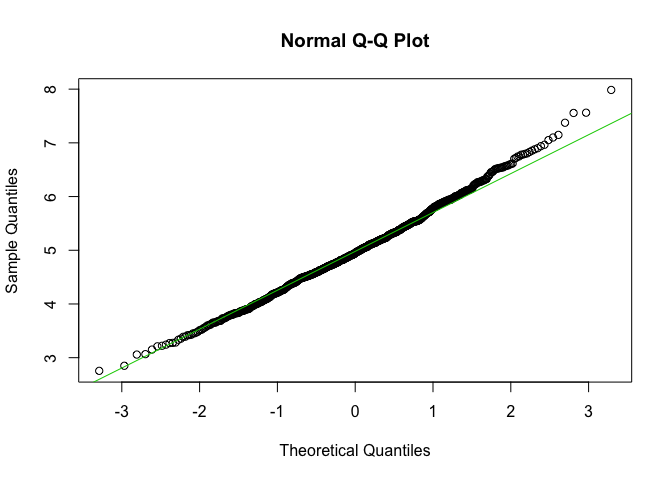
\includegraphics{part2_files/figure-latex/plot1-1} \end{center}

\subsection{Data Summary}\label{data-summary}

\begin{Shaded}
\begin{Highlighting}[]
\KeywordTok{summary}\NormalTok{(ToothGrowth)}
\end{Highlighting}
\end{Shaded}

\begin{verbatim}
##       len        supp         dose      
##  Min.   : 4.20   OJ:30   Min.   :0.500  
##  1st Qu.:13.07   VC:30   1st Qu.:0.500  
##  Median :19.25           Median :1.000  
##  Mean   :18.81           Mean   :1.167  
##  3rd Qu.:25.27           3rd Qu.:2.000  
##  Max.   :33.90           Max.   :2.000
\end{verbatim}

\begin{Shaded}
\begin{Highlighting}[]
\KeywordTok{table}\NormalTok{(ToothGrowth$supp,ToothGrowth$dose)}
\end{Highlighting}
\end{Shaded}

\begin{verbatim}
##     
##      0.5  1  2
##   OJ  10 10 10
##   VC  10 10 10
\end{verbatim}

\subsection{Comparison of Tooth Growth by Supp and
Dose}\label{comparison-of-tooth-growth-by-supp-and-dose}

Based on the box plot generated earlier, OJ appears to be doing better
with dose 0.5 and 1 on tooth growth than VC. To test this hypothesis by
hold a the mean of OJ and VC does not cross zero.

\subsubsection{Dose 0.5:}\label{dose-0.5}

We are 95\% confident that the limits of 1.719057 and 8.780943 actually
do contain the difference between the two population means. Because
those limts do not contain zero, this confidence interval suggests that
it is very possible that the two population means are not equal.

\begin{Shaded}
\begin{Highlighting}[]
\NormalTok{ojdose0}\FloatTok{.5} \NormalTok{<-}\StringTok{ }\NormalTok{ToothGrowth %>%}\StringTok{ }\KeywordTok{filter}\NormalTok{(supp==}\StringTok{"OJ"} \NormalTok{&}\StringTok{ }\NormalTok{dose==}\StringTok{"0.5"}\NormalTok{)}
\NormalTok{vcdose0}\FloatTok{.5} \NormalTok{<-}\StringTok{ }\NormalTok{ToothGrowth %>%}\StringTok{ }\KeywordTok{filter}\NormalTok{(supp==}\StringTok{"VC"} \NormalTok{&}\StringTok{ }\NormalTok{dose==}\StringTok{"0.5"}\NormalTok{)}
\KeywordTok{t.test}\NormalTok{(ojdose0}\FloatTok{.5}\NormalTok{$len,vcdose0}\FloatTok{.5}\NormalTok{$len)}
\end{Highlighting}
\end{Shaded}

\begin{verbatim}
## 
##  Welch Two Sample t-test
## 
## data:  ojdose0.5$len and vcdose0.5$len
## t = 3.1697, df = 14.969, p-value = 0.006359
## alternative hypothesis: true difference in means is not equal to 0
## 95 percent confidence interval:
##  1.719057 8.780943
## sample estimates:
## mean of x mean of y 
##     13.23      7.98
\end{verbatim}

\subsubsection{Dose 1:}\label{dose-1}

We are 95\% confident that the limits of 2.802148 and 9.057852 actually
do contain the difference between the two population means. Because
those limts do not contain zero, this confidence interval suggests that
it is very possible that the two population means are not equal.

\begin{Shaded}
\begin{Highlighting}[]
\NormalTok{ojdose1 <-}\StringTok{ }\NormalTok{ToothGrowth %>%}\StringTok{ }\KeywordTok{filter}\NormalTok{(supp==}\StringTok{"OJ"} \NormalTok{&}\StringTok{ }\NormalTok{dose==}\StringTok{"1"}\NormalTok{)}
\NormalTok{vcdose1 <-}\StringTok{ }\NormalTok{ToothGrowth %>%}\StringTok{ }\KeywordTok{filter}\NormalTok{(supp==}\StringTok{"VC"} \NormalTok{&}\StringTok{ }\NormalTok{dose==}\StringTok{"1"}\NormalTok{)}
\KeywordTok{t.test}\NormalTok{(ojdose1$len,vcdose1$len)}
\end{Highlighting}
\end{Shaded}

\begin{verbatim}
## 
##  Welch Two Sample t-test
## 
## data:  ojdose1$len and vcdose1$len
## t = 4.0328, df = 15.358, p-value = 0.001038
## alternative hypothesis: true difference in means is not equal to 0
## 95 percent confidence interval:
##  2.802148 9.057852
## sample estimates:
## mean of x mean of y 
##     22.70     16.77
\end{verbatim}

\subsubsection{Dose 2:}\label{dose-2}

We are 95\% confident that the limits of -3.79807 and 3.63807 actually
do contain the difference between the two population means. However,
because those limts do contain zero, this confidence interval suggests
that it is very possible that the two population means are equal.

\begin{Shaded}
\begin{Highlighting}[]
\NormalTok{ojdose2 <-}\StringTok{ }\NormalTok{ToothGrowth %>%}\StringTok{ }\KeywordTok{filter}\NormalTok{(supp==}\StringTok{"OJ"} \NormalTok{&}\StringTok{ }\NormalTok{dose==}\StringTok{"2"}\NormalTok{)}
\NormalTok{vcdose2 <-}\StringTok{ }\NormalTok{ToothGrowth %>%}\StringTok{ }\KeywordTok{filter}\NormalTok{(supp==}\StringTok{"VC"} \NormalTok{&}\StringTok{ }\NormalTok{dose==}\StringTok{"2"}\NormalTok{)}
\KeywordTok{t.test}\NormalTok{(ojdose2$len,vcdose2$len)}
\end{Highlighting}
\end{Shaded}

\begin{verbatim}
## 
##  Welch Two Sample t-test
## 
## data:  ojdose2$len and vcdose2$len
## t = -0.046136, df = 14.04, p-value = 0.9639
## alternative hypothesis: true difference in means is not equal to 0
## 95 percent confidence interval:
##  -3.79807  3.63807
## sample estimates:
## mean of x mean of y 
##     26.06     26.14
\end{verbatim}

\subsection{Conclusion}\label{conclusion}

We are 95\% confident that dose 0.5 and dose 1 of OJ result in longer
tooth length than dose 0.5 and dose 1 of VC. However, at the highest
dose of 2, there is no statistically significant difference between the
effects of OJ and VC.

\end{document}
